\section{Evaluating Predictive Models}

\subsection{Finding Model Parameters}
In predictive modeling, a model is generally \textbf{trained} to minimize a loss function. The data used in this process is called the \textbf{training data} or \textbf{training set}. The variable (or variables) being predicted is called the target variable and the independent variables are often called predictors of features.
These terms replace regressand and regressors from more typical econometrics terminology, respectively. 
Model training is the process of finding the best (or attempting to find, as we will see later)  \textbf{parameters} of the model. 
For a linear regression the parameters are the intercept and slope coefficients. 

\begin{align}
\hat{y} &= \phi_0 + \phi_1x \tag{regression specification} \\
L(\phi) &= \sum_{i=1}^n (y-\phi_0 -\phi_1x)^2 \tag{loss or cost over training data}
\label{eq:linear-loss}
\end{align}

As we saw with the different performance metrics for classification, the choice of a loss function is consequential. It's better to have a tailored loss function for your exact use case.
If you are predicting with Price is Right rules, where the prediction as close the to the truth without going over wins, the least squares cost function for linear regression is a poor choice because it weights positive and negative residuals equally.
We will continue by focusing on the sum of squared error and its ordinally equivalent forms like MSE, nonetheless. 

Many models involve additional parameters that are not found by the training process. Instead the parameters must be chosen by the researcher. These are called \textbf{hyperparameters}.
With a fixed specification, there are no hyperparameters in linear regression. However, there are choices like the inclusion of quadratic or higher order polynomial terms. Thus, the order of your regression equation may be considered a hyperparameter, where a higher order also corresponds to greater model complexity. 
Using your data to tune these hyperparameters requires care. We'll discuss accepted approaches in the validation section. 

\subsection{Training vs Test}

A fundamental principle in predictive modeling is that a model's performance should be evaluated on data that was not used during training. This avoids an optimistic bias from the training data and is a more honest test of how the model will perform in the wild, on new data. 

The test data serves this purpose. It consists of observations that are completely withheld from the model training process. For cross-sectional data, the test set should be determined by taking a random subset of the data. For time series data, you should select a longitudinal holdout where the test observations occurred after the training observations.  
Once the model parameters are estimated using only the training data, the model's performance is evaluated on the test data to provide an estimate of how well it will generalize to future observations.

This separation is necessary because models can achieve perfect fit on their training data simply by memorizing the noise, a phenomenon known as \textbf{overfitting}. 
This is bad in the same way that it is bad for schoolteachers to ``teach to the test'' instead of preparing students to apply their knowledge in a real setting. 

A model that overfits will show excellent performance on training data but poor performance on new data. By evaluating on test data, we obtain a more realistic assessment of the model's true predictive capability.

The test set should only be used for final evaluation, never for making decisions about model specification or parameter tuning. Using test data to guide modeling choices compromises its role as an unbiased evaluation metric.
This is a tradeoff. If, because of data scarcity, you would prefer to use additional data for training instead of testing, that is defensible but it comes at the cost of having an unbiased measurement of model error. 

\section{Validation}

\cite{neunhoeffer2019cross} notes the many uses of the term cross validation in the political science literature. The two most focal uses are for (1) getting an estimate of the true model error
and (2) for model tuning/selection. The latter is more common and this is our focus in these notes. We discuss simple holdout validation to establish some important ideas and then discuss the common $k$-fold approach. 


\subsection{Simple Holdout Validation}

Simple holdout validation addresses the challenge of model selection when multiple model specifications are under consideration. 
The basic approach randomly divides the available data into three distinct sets: training, validation, and test.

The training set is used to estimate model parameters for each candidate specification. 
The validation set (also called the development set) is used to evaluate the performance of each trained model. 
The model specification that achieves the best performance on the validation set is selected as the final model. 
Finally, the test set provides an unbiased estimate of the selected model's expected performance on new data.

A plausible allocation is to use 60\% of the data for training, 20\% for validation, and 20\% for testing, though these proportions may be adjusted based on the total sample size and the complexity of the models being considered, and the effect sizes of interest.

Each data subset serves a distinct purpose. The training set optimizes parameters, the validation set guides \emph{model selection}, and the test set provides final evaluation. 
This three-way split prevents the optimistic bias that would result from using the same data for both model selection and performance evaluation. If we did not include the validation set, we would either have to perform model selection with the training set or the test set. Performing model selection with the training set we know will lead to overfitting. 
Performing model selection with the test set biases the test set as a true measure of model error. 


When data is limited, this approach can be wasteful since a substantial portion of observations are held out from training. With $k$ points used for validation, the optimistic bias is greater for small $k$. But increasing $k$ means the overall error rate increases because we have fewer training points and thus more variance in the model. 

\begin{center}
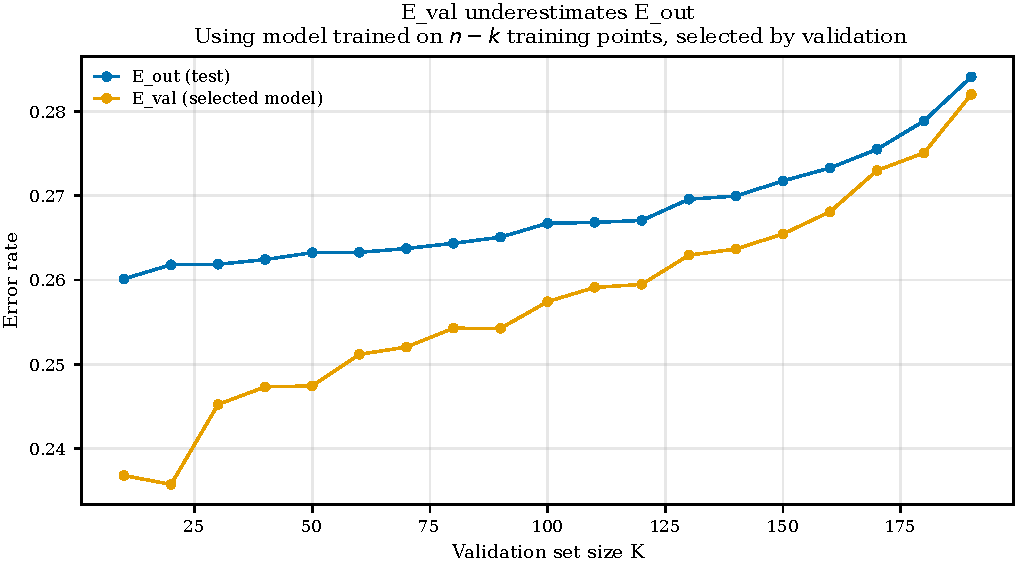
\includegraphics[width=.9\textwidth]{images/line_simple_holdout_validation_k.pdf}
\end{center}

In such cases, cross-validation techniques may be preferred to make more efficient use of available data.


\subsection{Cross Validation}

With scarce data and enough computing power, cross validation is often preferred, where we rotate the data through training and validation sets. Specifically in $\mathbf{k}$-\textbf{fold} validation,

\begin{enumerate}
\item Randomly split the data in $k$ partitions, or folds, of equal size.
\item Choose $k-1$ folds for training.
\item Use the remaining fold for validation--for a measure of performance.
\item Repeat 2-3 so that each fold is used as a validation set.
\item Compute the cross-validation estimate as the size-weighted mean of the fold-level validation errors. If folds are equal size, this reduces to the simple average.
\begin{equation}
\widehat{\mathrm{CV}}=\sum_{k=1}^K \frac{n_k}{N}\,\mathrm{Err}_k
\label{eq:cross-validation}
\end{equation}
\end{enumerate}

There is a sort of bias variance tradeoff in choosing $k$. If $k$ is small, your final performance estimate is pessimistic because the model is trained on relatively few data points. If $k$ is large (for instance, in the extreme of $k=n$, leave-one-out cross validation), then there is less bias but higher variance. $k$ between 5 and 10 is usually recommended.
   
Let's revisit the tradeoff in the size of the validation set in the case of simple holdout validation. 
Cross validation reduces the rise in test error you saw when the validation set size grew (because each fit keeps most data) and 
reduces selection bias (because the validation estimate averages over the held out folds).

This will generally give you a good measure of your model's performance on new data \textit{as long as you aren't using this for model selection.} \cite{varma2006bias} shows cross validation is biased in this case, though this isn't made especially clear in ESL and other texts.

\subsection{Nested Cross Validation (For Model Selection and Model Performance)}

In nested cross validation, we use two layers of cross validation: an inner loop for model selection (hyperparameter tuning) and an outer loop for performance estimation. This approach provides an unbiased estimate of model performance while avoiding the model-selection bias discussed previously.

The process works as follows:

\begin{enumerate}
\item \textbf{Outer Loop} (Performance Estimation):
   \begin{itemize}
   \item Split data into $K_{\mathrm{outer}}$ folds
   \item For each outer fold $k = 1, ..., K_{\mathrm{outer}}$:
     \begin{itemize}
     \item Hold out fold $k$ as the test set
     \item Use the remaining $K_{\mathrm{outer}} - 1$ folds for the inner loop
     \end{itemize}
   \end{itemize}

\item \textbf{Inner Loop} (Model Selection):
   \begin{itemize}
   \item Split the training data (from outer loop) into $K_{\mathrm{inner}}$ folds
   \item For each hyperparameter configuration:
     \begin{itemize}
     \item Perform $K_{\mathrm{inner}}$-fold cross validation
     \item Calculate average validation performance
     \end{itemize}
   \item Select the best hyperparameter configuration
   \item Retrain model with best hyperparameters on all inner loop data
   \end{itemize}

\item \textbf{Evaluation}:
   \begin{itemize}
   \item Test the model from step 2 on the held-out outer fold
   \item Repeat for all outer folds
   \item Report the average performance across all outer folds as the final estimate
   \end{itemize}
\end{enumerate}

Note, your average performance measure might average over models with different hyperparameter and can only be interpreted as the performance of your general algorithm.

%In my experience in industry, a degenerate case of nested cross validation is the most common. $K_{\mathrm{outer}}$ is usually set to one, so this is just cross-validation over a training+dev set and with a test set that is left untouched until after you have selected your model. This also makes it easier to decide what hyperparameters you should actually pick if you're deploying a model.

\subsubsection{Why Nested Cross Validation?}

Nested CV solves the problem of validation set error being optimistic. As noted in the \link{https://scikit-learn.org/stable/auto_examples/model_selection/plot_nested_cross_validation_iris.html}{scikit-learn documentation}, 
\begin{quotation}
\noindent Nested CV estimates the generalization error of the underlying model and its (hyper)parameter search. Choosing the parameters that maximize non-nested CV biases the model to the dataset, yielding an overly-optimistic score.
\end{quotation}

Nested cross validation separates the concerns of estimating model error and tuning:
\begin{itemize}
\item The inner loop finds the best hyperparameters for each outer training set
\item The outer loop provides an unbiased estimate of how well this model selection procedure works on truly unseen data
\end{itemize}


\section{Cross Validation The Wrong and Right Way}

This is adapted from ESL 7.10.2. Suppose you are facing a regression problem with many candidate predictor variables. Here is a \emph{bad} procedure:

\begin{enumerate}
   \item Screen the predictors. Find the predictor that is most correlated with the target. 
   \item Using just this predictor, build fit a polynomial curve to the data using linear regression. 
   \item Use cross-validation to find the best polynomial order. 
\end{enumerate}

Let's see how this works using American Time Use Survey data. First, we use only the 2024 data. 

\begin{lstlisting}
import pandas as pd
import numpy as np

df = pd.read_csv("atussum_2024.dat")

# TRERNWA is a weekly earnings variable
df = df[df['TRERNWA'] > 0]
income = df['TRERNWA']

# time use columns happen to start with lower-case t
time_use_columns = [c for c in df.columns if c.startswith("t")]
# there are 372 time use columns. a lot!

# find most correlated column
highest_correlation = 0
best_col = None
for col in time_use_columns:
    r = np.corrcoef(income, df[col])[0][1]
    
    if np.abs(r) > np.abs(highest_correlation):
        best_col = col
        highest_correlation = r

# t030405, waiting associated with caring for household adults is the most correlated    
\end{lstlisting}


